\documentclass[12pt]{report}
\title{System validation document}
\date{\today \\ Version 0.0.1}

\usepackage[latin1]{inputenc}
\usepackage{amsmath}
\usepackage{graphicx}
\usepackage{a4wide}
\usepackage{enumitem}
\usepackage{url}
\usepackage{caption}
\usepackage[parfill]{parskip}
\usepackage{appendix}
\usepackage{subcaption}
\usepackage{color}
\usepackage{booktabs}
\usepackage{lineno}
\usepackage{float}
\usepackage{longtable}
\usepackage{colortbl}
\usepackage{amsfonts}
\newcounter{counter}

%\linenumbers
\modulolinenumbers[5]

\begin{document}
	\begin{titlepage}
		\begin{center}
			\textsc{\Large EINDHOVEN UNIVERSITY OF TECHNOLOGY}\\[1.5cm]
			
			\textsc{\Large System Validation}\\[0.8cm]
			\hrule
			\vspace{0.5cm}
			{ \huge \bfseries EUV Wafer Stepper \\[0.4cm] }
			\hrule
			\vspace{1.5cm}
			\noindent
			\begin{minipage}[t]{0.5\textwidth}
				\begin{flushleft} \large
					\emph{Authors:}\\
					R.M. van den Hurk (0817761)\\
					Z. Ben Snaiba (0748095)\\
					P.M.M. van Wesel (0818131)\\
				\end{flushleft}
			\end{minipage}\\
			\vspace{5cm}
			\begin{minipage}[t][8cm]{0.3\textwidth}
				\begin{flushright} \large
					\today
				\end{flushright}
			\end{minipage}
			
			\vfill
			
		\end{center}
	\end{titlepage}
	
	\tableofcontents
	
	\chapter{System overview}
	
	\section{System overview}
	\begin{figure}
		\centering
		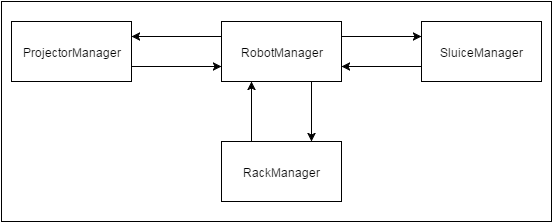
\includegraphics[scale=0.7]{schematicoverview}
		\caption{A schematic overview of the system}
		\label{fig:overview}
	\end{figure}
	The Extreme Ultraviolet (EUV) Wafer Stepper is a system developed by ASML to treat silicon wafers. Treating a wafer is the act of projecting an image with ultra violet light onto a silicon wafer. Since ultra violet radiation is absorbed by air, this treatment has to happen in a vacuum to ensure the accuracy of the projection. This means wafers will have to enter and exit the system through airlocks, also referred to as sluices. One robot will move wafers from the input to the airlocks or from the airlocks to the output for treated wafers from outside the vacuum chamber. One robot will move wafers from the airlocks to a buffer rack inside the vacuum chamber and vice versa for treated wafers. A last robot, located inside the vacuum chamber, takes wafers from the internal buffer rack to the projector and back once the projector is done. A schematic overview of the system can be found in figure \ref{fig:overview}.
	\section{System components}
	The system can be broken down into individual components to be considered by the software. These components are the following:
	\begin{itemize}
	\item \textbf{Input} - A rack containing untreated wafers located outside of the vacuum chamber.
	\item \textbf{Output} - A rack for treated wafers outside the vacuum chamber.
	\item \textbf{Airlocks} - An array of airlocks providing entrance into the vacuum chamber. Each airlock consists of an inner door, outer door, vacuum pump and air pressure sensor.
	\item \textbf{Buffer Rack} - The buffer rack located inside the vacuum chamber that can temporarily hold wafers.
	\item \textbf{Projector} - The projector inside the vacuum chamber that treats the wafers.
	\item \textbf{Robot A} - The robot that can reach \emph{Input}, \emph{Output} and the \emph{Airlocks}.
	\item \textbf{Robot B} - The robot inside the vacuum chamber that can reach the \emph{Airlocks} and \emph{Buffer Rack}.
	\item \textbf{Robot C} - The other robot inside the vacuum chamber that can reach the \emph{Buffer Rack} and \emph{Projector}.
	\end{itemize}
	
	\chapter{System requirements}
	
	\newcommand{\req}[1]{
		\item[\textbf{R\stepcounter{counter}\arabic{counter}}] {#1}
		\hrule
	}
	
	\newcommand{\reqb}[2]{
		\item[\textbf{{#1}}] {#2}
		\hrule
	}
	
	\section{Liveness requirement}
	\begin{itemize}
		\req{If the system is operating normally, an untreated wafer on the input rack will enter the system, and exit the system after it has been treated.}
	\end{itemize}
	
	\section{Sluice requirements}
	\begin{itemize}
		\req{Only one sluice door can be open at a time.}
		\req{The outer sluice door can only open if there is normal air pressure inside the sluice.}
		\req{The inner sluice door can only open if there is a vacuum inside the sluice.}
		\req{The vacuum pump can only make a vacuum if both sluice doors are closed.}
		\req{The doors of a sluice can not close if a robot is reaching inside.}
	\end{itemize}
	
	\section{Sluice robot requirements}
	\begin{itemize}
		\req{Robot A may only move to a sluice if the outer door of the target sluice is open.}
		\req{Robot B may only move to a sluice if the inside door of the target sluice is open.}
		\req{Robot A\&B may only choose a sluice to put a wafer in that is empty.}
		\req{Robot A\&B may only try to retrieve a wafer from an occupied sluice.}
		\req{Robot A\&B can only put a wafer on an empty spot on the rack.}
		\req{Robot A\&B may only target functioning sluices.}
		\req{Robot A\&B should only try to take wafers from the rack if there are wafers available.}
		\req{Robot B may not access the same spot on the rack as Robot C at the same time.}
	\end{itemize}
	
	\section{Inside robot requirements}
	\begin{itemize}
		\req{Robot C can not access the same spot on the rack as Robot B at the same time.}
		\req{Robot C can not put a wafer on the projection platform when it is occupied.}
		\req{Robot C can not take a wafer from the projection platform if the projection is not done.}
		\req{Robot C can not put a wafer on an occupied place on the rack.}
	\end{itemize}
		
	\section{Projector requirements}
	\begin{itemize}
		\req{The projector only starts its treatment when a wafer is on the projection platform.}
	\end{itemize}
	
	\chapter{System interactions}
\section{User actions}
	\begin{itemize}
\item OpenOuterDoor(N) - Open the outer door of sluice N.
\item CloseOuterDoor(N) - Close the outer door of sluice N.
\item OpenInnerDoor(N) - Open the inner door of sluice N.
\item CloseInnerDoor(N) - Close the inner door of sluice N.
\item PumpVacuum(N) - Make a vacuum in sluice N.
\item ReleaseVacuum(N) - Release the vacuum in sluice N.

\item RobotFromInput - Robot A picks up a wafer from the input rack.
\item RobotToOutput - Robot A deposits a wafer on the output rack.

\item RobotToSluice( R, S ) - Robot R deposits the wafer it is holding in sluice S.
\item RobotFromSluice( R, S ) - Robot R picks up a wafer from sluice S.

\item RobotToRack( R, P ) - Robot R deposits the wafer it is holding to position P on the buffer rack.
\item RobotFromRack( R, P ) - Robot R takes a wafer from position P on the buffer rack.

\item RobotToProjector - Robot C deposits the wafer it is holding on the projector.
\item RobotFromProjector - Robot C picks up the wafer that is currently on the projector.

\item TreatWafer - The projector treats a wafer.
\end{itemize}

	\section{System properties}
	\begin{itemize}
\item IsOuterDoorOpen(N) - True if the outer door of sluice N is open false otherwise.
\item IsInnerDoorOpen(N) - True if the outer door of sluice N is open false otherwise.
\item IsVacuum(N) - True if there is currently a vacuum in sluice N false otherwise.
\item IsWaferInSluice(N) - True if there is a wafer is sluice N false otherwise
\item IsRobotInSluice(N) - True if there is a robot in sluice N false otherwise
\item IsRobotAccessingRack(R, N) -  True if robot R is currently accesing rack N.
\item IsWaferOnRack(R, P) - True if there is a wafer in rack R at position P false otherwise
\item IsWaferTreated - True if the wafer in the projector has been treated false otherwise
\item IsSluiceBroken(N) - Sluice N has failed to respond to a user action and will be marked as broken.
\item IsWaferInProjector - Whether there is a wafer in projector or not.
	\end{itemize}
	
	\chapter{Requirements in terms of interactions}
	\section{Liveness requirement}
	\begin{itemize}
		\reqb{SR1}{If a wafer appears at position p on the input rack, we should see the following sequence of actions. Other actions can happen between any two of these actions, provided they are not one of those two actions with different parameters.\\
		\begin{itemize}
\item robotTakeWafer( A, p )
\item robotWaferInSluice( A, s ) \emph{- For some arbitrary sluice s}
\item robotWaferFromSluice( B, s )
\item robotDepositWafer( B, p2 ) \emph{- For some arbitrary position p2 on the inner} rack.
\item robotTakeWafer( C, p2 ) \emph{directly followed by} robotCTreatWafer.
\item robotDepositWafer( C, p3 ) \emph{- For some arbitrary position p3 on the inner rack.}
\item robotTakeWafer( B, p3 )
\item robotWaferInSluice( B, s2 ) \emph{- For some arbitrary sluice s2.}
\item robotWaferFromSluice( A, s2 )
\item robotDepositWafer( A, p4 ) \emph{- For some arbitrary position p4 on the output rack.}
\end{itemize}
}
	\end{itemize}
	
	\section{Sluice requirements}
	\begin{itemize}
		\reqb{SR2}{openOuterDoor(N) if innerDoorOpen(N) is true.}
		\reqb{SR3}{openOuterDoor(N) vacuum(N) is false.}
		\reqb{SR4}{openInnerDoor(N) vacuum(N) is true.}
		\reqb{SR5}{pumpVacuum(N) outerDoorOpen(N) and innerDoorOpen(N) are both true.}
		\reqb{SR6}{
\begin{itemize}		
		\item closeOuterDoor(N) can only happen if robotInSluice(N) is false.
\item closeInnerDoor(N) can only happen if robotInSluice(N) is false.
\end{itemize}		
		}
	\end{itemize}
	
	\section{Sluice robot requirements}
	\begin{itemize}
		\reqb{SR7}{robotWaferInSluice(A,N) can only happen if outerDoorOpen(N) is true.}
		\reqb{SR8}{robotWaferInSluice(B,N) can only happen if innerDoorOpen(N) is true.}
		\reqb{SR9}{\begin{itemize}
		\item  robotWaferInSluice(A, N) waferInSluice(N) is false.
		\item robotWaferInSluice(B, N) waferInSluice(N) is false.
		\end{itemize}}
		\reqb{SR10}{
		\begin{itemize}
		\item robotWaferFromSluice(A, N) can only happen if  waferInSluice(N) is true
		\item robotWaferFromSluice(B, N) can only happen if waferInSluice(N) is true.
		\end{itemize}
		}
		\reqb{SR11}{RobotToRack( R, P ) can only happen after another RobotToRack( R, P ) with the same P, if a RobotFromRack( R, P ) has happened with the same P.}
		\reqb{SR12}{openOuterDoor(N), closeOuterDoor(N), openInnerDoor(N), closeInnerDoor(N), pumpVacuum(N), releaseVacuum(N), robotWaferInSluice(R,N),robotWaferFromSluice(R,N),outerDoorOpened(N), outerDoorClosed(N),innerDoorOpened(N),innerDoorClosed(N),vacuumDone(N) and vacuumReleased(N) can only happen if sluiceBroken(N) is false.}
		\reqb{SR13}{RobotFromRack( R, P ) can only happen if IsWaferOnRack( P ) is true for the same P.}
		\reqb{SR14}{RobotTakeWafer(B, p) or RobotDepositWafer(B, p) can only happen if robotAccessingRack(C,C\_Rack) is false.}	\end{itemize}
	
	\section{Inside robot requirements}
	\begin{itemize}
		\reqb{SR15}{RobotTakeWafer(C, p) or RobotDepositWafer(C, p) can only happen if robotAccessingRack(B,C\_Rack) is false. }
		\reqb{SR16}{robotCRetreiveWafer can only happen if waferInProjector is false.}
		\reqb{SR17}{robotCRetreiveWafer can only happen if waferTreated is true.}
		\reqb{SR18}{robotDepositWafer(C, N) can only happen if waferOnRack(C\_Rack, P) is true for some P.}
	\end{itemize}
	\section{Projector requirements}
	\begin{itemize}
		\reqb{SR21}{treatWafer can only happen after robotCTreatWafer if no robotCRetrieve happened after that.}
	\end{itemize}
	
	\chapter{System model}
	\section{Model overview}
	\begin{figure}
		\centering
		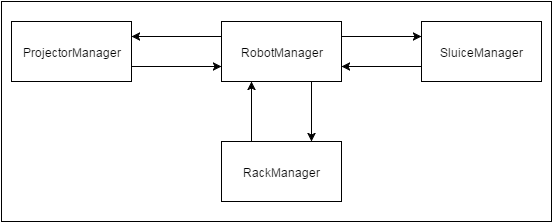
\includegraphics[scale=0.7]{schematicoverview}
		\caption{A schematic overview of the software components}
		\label{fig:components}
	\end{figure}
	To verify the system, a model of the software to be made. The software is split up into the following three components:
	\begin{itemize}
	\item \textbf{SluiceManager} - This component manages the sluices, it runs parallel for each sluice. The purpose of this component is to control the individual airlocks.
	\item \textbf{RobotManager} - This component manages the different robots in the system, and runs a parallel process for each robot.
	\item \textbf{ProjectorManager} - The projector is managed by this component.
	\end{itemize}
	
	A schematic view of this system can also be found in figure \ref{fig:components}.
	
	\section{Responsibilities}
	The purpose of this separation into components is to separate responsibilities of the system, increasing the cohesion and decreasing the coupling of the system. The different actions of the system can be divided over the different components to establish this separation of responsibilities.
	
	\subsection*{SluiceManager}
	\begin{itemize}
		\item OpenOuterDoor
		\item CloseOuterDoor
		\item OpenInnerDoor
		\item CloseInnerDoor
		\item PumpVacuum
		\item ReleaseVacuum
	\end{itemize}
	
	\subsection*{RobotManager}
	\begin{itemize}
		\item RobotFromInput
		\item RobotToOutput
		\item RobotToSluice
		\item RobotFromSluice
		\item RobotToRack
		\item RobotFromRack
		\item RobotToProjector
		\item RobotFromProjector
	\end{itemize}		
	
	\subsection*{ProjectorManager}
	\begin{itemize}
		\item TreatWafer
	\end{itemize}
	
	\section{Formal model}
	

\end{document} 